%%%%%%%%%%%%%%%%%%%%%%%%%%%%%%%%%%%%%%%%%%%%%%%%%%%%%%%%
%
% Change the option between square brackets
% depending on the document you have to write:
%
% proposal    for the initial proposal
% review      for the literature review
% progress    for the progress report
% final       for the final report
% 
%%%%%%%%%%%%%%%%%%%%%%%%%%%%%%%%%%%%%%%%%%%%%%%%%%%%%%%%
\documentclass[final]{cmpreport}
\makeatletter
\input{t1pcr.fd}
\makeatother
\setlength{\footnotesep}{3ex}

% Some package I am using. You may not need them
%
\usepackage{rotating}
\usepackage{subfloat}

%\setkeys{Gin}{draft}
\title{Raspberry Pi Smart Home and Progressive Web App}
\author{Vincenzo Mann}
\registration{100121797}
\supervisor{Dr Ben Milner}
\ccode{CMP-6013Y}

% commands

\newcommand{\pwa}{Progressive Web App}
\newcommand{\rpi}{Raspberry Pi}
\newcommand{\rtd}{Realtime Database}
\newcommand{\has}{Home Automation System}
\newcommand{\refff}{(NEEDS REFERENCE!)}
\newcommand{\iot}{Internet of Things}

% needs 
\summary{
\has{}s (HASs) have changed a lot over the decades to suit the needs of the modern smart home. Smart homes today frequently use the \iot{} (IoT) to connect physical household objects over the internet network, where users can interact with via a mobile/device application or website. \pwa{}s (PWAs) are an exciting new web technology that provide offline functionality and a native app feeling. PWAs open up a range of new possibilities and have the potential to change the way people use applications and the internet. Combining home automation with PWAs could improve the functionality and widespread use of smart homes. Three real-world problems that HASs try to provide solutions for are the environment, health and security \cite{futureofsmarthomes}. This project will aim to evaluate the feasibility and suitability of using a PWA to control a smart home and reflect it against how well it could solves these problems.
}

\acknowledgements{
Thank you to Dr Ben Milner for his support and advise during this project.
}

\nolist
\onePageLists
\linespread{1.5}

\begin{document}

%---------------------------------
%	PROJECT DESCRIPTION SECTION
%---------------------------------

\section{Introduction}\label{introduction}

    \subsection{Aims}
    
    The main aims of the project:

    \begin{enumerate}
        \item Develop a HAS which can manually and autonomously control electronics within a scaled-down model simulating a house.
        \item Design and engineer a PWA which allows a user to interact and control the hardware features of the system.
        \item Assemble hardware components that will be compatible with the RPi single-board computer to create a functioning system.
        \item Evaluate the affect of using a PWA with a HAS compared to existing methods and how the system could help issues with current HASs in the real world.
    \end{enumerate}

    \subsection{Motivation}

    Embedded systems are a key part in the ``Internet of Things'' which is where innovative and exciting new technology is happening and moving more towards; HASs are a common application of IoT. PWAs are a very new technology and will probably change the way the world uses apps and websites, therefore designing and experimenting with what it can do will be a beneficial investment of time. If a PWA controlled smart home were introduced to the industry then this could become an impactful way to help real-world problems such as reducing carbon emissions and aiding those that require health supervision.
    
    \subsection{Report Structure}
    
    % TO DO - GIVE DESCRIPTIONS.

    Section 2 - Context and Research.\\
    Section 3 - Project Description and Rationale.\\
    Section 4 - System Design.\\ 
    Section 5 - System Implementation.\\ 
    Section 6 - System Evaluation.\\ 
    Section 7 - Conclusion.\\ 
    References\\ 
    Appendix - Project Gantt Chart
   
    %\subsection{Acronyms}

\section{Context and Research}\label{context}

    % TO DO - SHOW YOU ARE AN EXPERT IN THE FIELD

    \subsection{Home Automation Systems}\label{iot}

    The IoT is the principle of a network of physical objects being connected to each other over the internet network to work together and improve the lives of humanity. Many IoT products are examples of embedded systems that aim to perform technological tasks whilst out of sight and mind of users. Home automation is an example of an embedded system but has increasingly been combined with IoT to create a more powerful solution. HAS, also referred to as smart-homes, are environments with ambient intelligence and automatic control that respond to the behaviour of the resident with various services \citep{lossofauto}.
    % TO DO - MORE DETAIL. WHAT CAN BE AUTOMATED? MORE EXAMPLES AND CONTEXT
    
    % TO DO - EXISTING HAS. WHAT'S BEEN DONE? WHAT TECH IS USED?

    IoT also has the capability of collecting vast amounts of data which can be used for data analysis to predict certain outcomes. This is a useful tool for smart-cities and corporations to gain insight to the energy consumption and behaviour of smart-home owners \citep{IoTBigData}, whether that is for better or worse will be discussed in the following sections.

    \subsection{Issues that Smart Homes Aim to Solve} 

    \cite{futureofsmarthomes}, \cite{smarthomecomms}, \cite{iotehs} and many others focus on three main benefits that home automation provides for; environment, health and security.

    % environment
    The world is much more conscious about being environmentally friendly. A practical way for everyone to do their bit is by reducing how much energy they use in their household and/or reducing how much energy is wasted. Smart meters improve power efficiency control to help reduce negative impacts on global warming and save the user money in the process.
    % TO DO - HOW DO THEY DO THIS?
    % TO DO - MORE DETAIL AND EXAMPLES

    % health
    The design of smart homes would have significant impact on the living standards for the elderly and disabled. The world population is aging and urges to have the infrastructure in place to help monitor and assist those who require constant medical attention, as well as improve quality of life when living independently.
    % TO DO - HOW WOULD THESE HELP?
    % TO DO - MORE DETAIL AND EXAMPLES

    % security
    Real-time alarm generation gives extra comfort knowing the user can track the status of the house security, such as if the door has been opened and if it is someone with authority to do so. Video analysing techniques, such as face recognition, is one of the most practical security measures as it has the ability to distinguish occupants and strangers. Embedded sensors are another way of monitoring activity or assisting to prevent unfortunate events. 
    % TO DO - MORE DETAIL AND EXAMPLES

    \subsection{Issues with Smart Homes}

    It is ironic how one of the major purposes that smart homes set out to solve is one of its biggest flaws. A common conclusion was that smart homes were a violation of privacy and a vulnerability to cyber crime. \cite{iotlegislation} highlights why IoT requires a regulatory framework to address the societal impact of current legislation. Most journals gave significant attention to the advantages to IoT but little to the potential threats. However, journals that do review the drawbacks focus its entire attention on the limitations; specifically all pointing to the fault of lack of standards. \cite{PrivacyImpact} makes the conclusion that the HASs that provide security do not necessarily provide privacy; this is worrying when there are large quantities of Personally Identifiable Information (PII) collected from these IoT systems. A case study by \cite{smartplug} into smart plug security vulnerabilities, also exclaims to raise awareness of danger with the increasing use of IoT and smart home technologies. It is clear that there are no set guidelines or standards for designing and implementing an IoT system that truly protects the user from being exploited, though there are many researchers with various proposals.
    
    \subsection{Existing Solutions}
    
    % TO DO - NEEDS REALLOCATING AND EDITING
    A common method of developing real-life home automation is to use Zigbee to wirelessly communicate household objects in a mesh network. There are also a large quantity of projects that use a Raspberry Pi for both real and simulated HASs. As examples, \cite{homeiot} produces a Zigbee-based real HAS and \cite{androidhas} produces a web-based simulated HAS. This project will be an example of the latter just to demonstrate the principles of a smart home but it will be powered through a Raspberry Pi as it is a suitable controller for this project and has been tried and tested on countless other projects of similar scope. The difference being with this project is that it will use a PWA. 
    % TO DO - MORE DETAIL AND EXAMPLES
    
    \subsection{Progressive Web Apps}
    
    % TO DO - EDIT, MORE DETAIL AND EXAMPLES. link to tech selection. COMPARE TO OTHER APP METHODS
    A PWA allows users to control from anywhere; it is responsive to different devices, it can use push notifications and it has some functionality offline through the use of service workers \citep{pwa}. Therefore, it fulfills all the requirements that a web app can deliver plus the benefits of being much more flexible. Although much research has gone into combining HASs with web and mobile applications, there has not been much into HASs with PWAs.
    
    
\section{Project Description and Rationale}

This project will be the initial prototype of the system, however, information required to complete the final version of the project will be fully documented so that project can be continued.

Upon successful completion of this project, a system will be produced that will allow users to electronically monitor and control their household environment. The user will interact with the system through a PWA interface which can be accessed by any electronic device that utilises a web browser. The PWA communicates with a Raspberry Pi micro-controller that provides the logical operations for the sensors and actuators fitted in the household environment. The PWA will display live feedback from the sensors and provide control options for the actuators.

This project will aim to evaluate the feasibility and suitability of using a PWA to control a smart home and reflect it against how well it could solve real-world challenges with health, security and the environment. The following subsections describe which sensors and actuators best demonstrate the three categories. 

    \subsection{Environment}
    
    % justify environmental temp/light sensor => leds
    A UK government report \citep{ukenergy} stated that ``In 2017, the domestic sector accounted for 28 per cent of total final energy consumption''. This statistic emphasises the importance of monitoring energy consumption and proves why it is a main focus of smart homes. Controlling and setting limits on energy consumption from heating and lighting is an effective solution. A temperature and lux sensor will be implemented to display the real-time light and temperature values on the app. The app will allow the user manually vary the intensity of lights and turn heating either on or off. The user can set the threshold value for when the lights and heating should become active and active. This system will use LEDs to represent the lighting and heating.

    \subsection{Security}
    
    % justify security - monitor/door sensor => alert
    \cite{evaluateiotsecurity} states the ``most vulnerable level of the IoT system model is the perception layer due to the physical exposure of IoT devices''. This includes sensors for data collection such as Radio-Frequency Identification (RFID) which have various opportunities to compromise the security. Therefore, it is important to avoid or mitigate security threats from the perception layer in the proposed system. For this reason, this project will avoid using technologies that could be compromised, e.g. gaining unauthorised access to the property. This system will only automate the notification to the user of potential intruders by using a motion sensor and magnetic door alarm. This is not technically home automation as it is not controlling any device, only sensing. However, compared to existing HASs it has been shown that there is high risk in compromising security when automation is introduced for security purposes.
    
    \subsection{Health}
    
    % justify health pulse sensor => monitor/999
    ``The global market for Internet of Things (IoT) sensors in health care totaled \$1.1 billion in 2017 and is estimated to reach \$1.9 billion by 2022, growing at a compound annual growth rate (CAGR) of 12.7\% for the period of 2017-2022'' \citep{sensorsinhealthcare}. There are different ways in which a smart home can provide health care; \cite{lossofauto} stress the need for assistance for people with loss of autonomy (LOA), whereas \cite{elderlydisabled} argue that medically monitoring the health of residents with serious conditions is most crucial. This web based solution has the potential and scope to remotely perform physical tasks to aid those with LOA e.g. opening blinds. However, this system will instead focus on monitoring the health of the resident because it will demonstrate a wider range of functionality and capability of the system and how a smart home can be a life-saving service in the real world. There will be a heart rate pulse sensor which can display and track the user's health and will simulate the act of automatically alerting specified contact numbers or emergency services when immediate medical attention is required.   

\section{System Design}\label{design}

The design of the system has been developed by starting with the end goal/product and working backwards. A prioritised list of system requirements has been formulated to meet the objectives of the project. The specifics of each requirement are oriented around the user's experience because the system is only as effective as the time it is used for. These requirements are then used to determine which tools and technology are best suited to complete the tasks. It must then be figured out how these technologies work and how they will work together. Finally, designing the technical plan of implementation.

    \subsection{System Requirements}
        
        \subsubsection{Use Cases}
        
        Figure~\ref{figUse} represents the basic use cases of the system. This includes the requirement that the user can register and log in. When the user reads the sensor data offline, they can control and change the data but it will not come into action until the app is online and synchronised with the RPi.
        
        %Use Case Diagram
        \begin{cmpfigure}[htb]{Use Case diagram of the system.\label{figUse}}
    	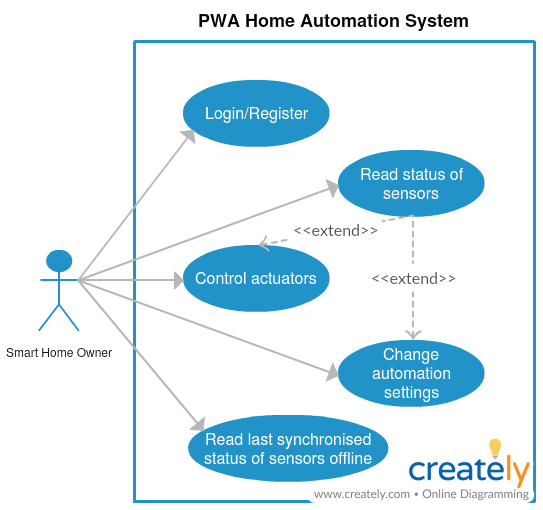
\includegraphics[width=0.6\textwidth]{Use_Case.png}
        \end{cmpfigure}
    
        \subsubsection{MoSCoW Analysis}
        
        To properly design the software, the initial requirements must be well stated and it must be made clear what requirements are within or outside the scope of the project. For that reason a MoSCoW requirement analysis is good for building the fundamentals first. Through agile development, these requirements can adapt but it ensures the build is going down the correct path. It is also important to include any assumptions as these can become increasingly difficult to resolve towards the end of the life-cycle. 
        
        \textbf{Must Have:}
        
        The PWA interface must communicate with the RPi from an external device via the internet.
        
        The PWA must display the HAS information and have basic functionality offline.
        
        The RPi must communicate with the electronic components of the HAS.
        
        The HAS must display the temperature reading and be able to set the temperature target for the ``Heating'' LED to activate automatically and manually.
        
        The HAS must display the light reading and be able to set the light target for the ``Lighting'' LED to activate automatically and manually.
        
        The HAS must display the pulse reading, be able to set the heart rate boundaries and the contact number for the system to automatically send an emergency SMS when the pulse value go outside the boundary.
        
        The HAS must display the motion reading and alert the user when there is activity.
        
        The HAS must display the door status and alert the user when the door has been opened.
        
        \textbf{Should Have:}
        
        The PWA should have a user friendly and easy to use UI.
        
        The PWA should have a registration and log-in for each user.
        
        \textbf{Could Have:}
        
        The HAS could have multiple sensors such as motion sensors for different rooms to display which rooms have triggered the motion sensors.
        
        The PWA could have a user manual for instructions and troubleshooting.
        
        The HAS could make use of motors to perform physical tasks e.g. opening blinds, to aid those with LOA.
        
        \textbf{Won't Have:}
        
        The HAS won't have any automation of security such as RFID.
        
        \textbf{Assumptions:}
        
        There is only one user per HAS.
        
        \subsubsection{Limitations}
        
        The system doesn't account for troubleshooting problems with the hardware, such as a loose connection. The hardware should be closed-off to the user so there is not much they can do without the assistance of an engineer. 
        The system is reliant on the RPi being set up and configured properly which can be quite technical and would also require assistance from an engineer or very technical instructions.
        
    \subsection{Technology Selection}
    
    % what, why?
        
        \subsubsection{Application: PWA}
        
        % link to research section. maybe beef up context and just refer to it
        
        PWAs are chosen for the application for their versatility. As it is simply just a website it can be used on any device with a web browser, and multiple devices at once. A website also means the app doesn't have to be re-coded in different languages to support different platforms/devices and the user doesn't need to download or install anything but still gets the look and feel of a native app. PWAs even support mobile push notifications and home-screen shortcut icons. The main selling point though is their ability to maintain some app functionality whilst offline through the use of service workers caching data and background syncing. % explain?
        
        % react language - suits pwas, ui, redux, firebase
        
        \subsubsection{Database: Firebase}
        
        The Firebase API is a web application development platform developed by Google which has many functions. This project will make use of its Realtime Database to manage the synchronisation of data from the PWA and the RPi client. The system will also use Firebase to host the website, Firebase can also to provide authentication and security which will be useful for this project. In addition to PWAs use of service workers, Firebase will enhance the offline functionality of the PWA as it provides offline support using a local database on the device (no SQL required) so the system functions smoothly when there is no network connection available. 
        
        % firestore, authentication, hosting
        
        \subsubsection{Micro-controller: RPi}
        
        The Raspberry Pi 3 Model B will be the core processing controller for the electronic components.
        
        % python
        
        \subsubsection{Hardware}
        
        % parts list

    \subsection{System Architecture}
    
    % how work together?
    
    % interfaces 

    The model of this system has three main parts: the PWA, the RPi and the Firebase Realtime Database (FRD).
    
    Figure~\ref{figClass} represents the communication data flow and the classes of the system. The class diagram has a one-to-one relationship, however, with the potential implementation of multiple users the diagram would include a User class as child of the FRD with a one FRD to many Users relationship.
    
    %Class Diagram
    \begin{cmpfigure}[htb]{Class diagram and communication flow of the system.\label{figClass}}
	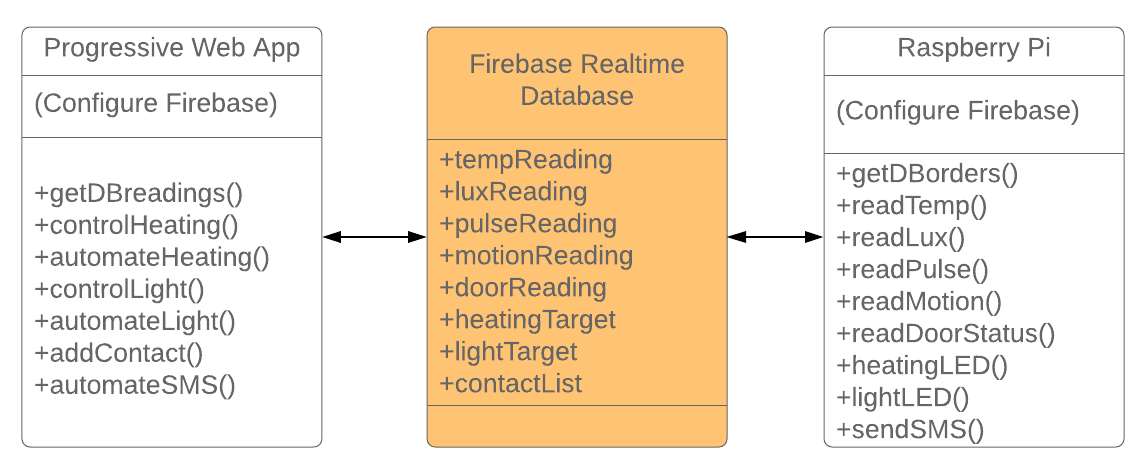
\includegraphics[width=\textwidth]{Class_Diagram.png}
    \end{cmpfigure}
        
    \subsection{PWA} % designing pwa - technical
    
    The PWA is the user interface (UI) for remote operation and control of the system from multiple devices. The website will be set up using Node.js and Firebase Hosting. The PWA communicates with the FRD via JavaScript; the UI lets the user view and update the data which will consequently cause the RPi to react accordingly, e.g. changing the ``Heating'' LED brightness value.
    
    % insert UI drawing
    
    % pseudo code
    
    % service workers
    
    \subsection{Firebase} % designing firebase - technical
    
    % firebase is the shared key/resource. other two just push/pull from firebase
    % database structure
    % what data for firestore and what for rtd from which locations
    
    
    \subsection{Raspberry Pi} % designing rpi - technical
    
    % pseudo code why python
    % script for each sensor, interrupts
    % controlling gpio, interfaces
    
     There will be a python script configured with the FRD using the Pyrebase and RPi GPIO imports. The script sends the status of the sensors to the FRD to display on the PWA and the script receives data from the FRD and uses the data to control the GPIO.
    
    \subsection{Hardware} % designing hardware - technical
    
    % gpio shield required for adc, easier gpio output
    % no external voltage requires
    % led for each sensor
    The hardware and circuitry will not be complicated for this project. Breakout boards will be used for the sensors rather than building them from scratch and LEDs are the only electronic actuators which are very easy to control. The circuit will be developed using a prototyping solderless breadboard; the final model may still use a breadboard but preferably a copper clad board will be made with the components soldered on. This will help improve transportation of the model and make it easier to fit components inside the model. 
    
        \subsubsection{Circuit Design}
        % fritzing design?
    
\section{System Implementation}

% introduce implementation section

    \subsection{Development Methodology}
    
    Each electronic component will be tested and run individually before being compiled into one circuit to ensure all components are compatible and working as expected. This will reduce the complexity of debugging when testing the entire system. A multimeter will be used to test the continuity of the circuit. A RPi online simulator might also prove a useful tool to test a different circuit to the current one in development without taking it apart. 
    
    A basic version of the app will be created to start with and will gradually implement one function at a time to test and debug it thoroughly. Once the link between the app and the RPi has been established, the app will test controlling each component individually. When the entire system has been built, it will undergo a full test to find any remaining bugs; this will be done by using the system in unorthodox ways a user would interact with the app as well as the standard use cases. Software will include error handling to provide helpful information and warnings to the user. Error handling will also help troubleshooting whilst in development. The software will be coded using VS Code IDE which has inbuilt debugging tools. The PWA development will make use of the Google Chrome Developer Tools to diagnose problems and Lighthouse to test and analyse PWA functionality. 
    
    % Git
    
    % Coding Standard
    
    % Project Plan - appendix
    
    \subsection{Web Application}
    % introduce web implementation
    % software and tools used eg chrome dev tools
    
        \subsubsection{React}
        % component based, store
        % setup, config and dependencies
        % file structure
        % code/algorithms
        
        \subsubsection{Redux}
        % setup, config and dependencies
        % createStore
        % reducers and actions
        % asynchronous functions
        % redux tools
        % code/algorithms
        % 
    
        \subsubsection{Firebase Authentication}
        % setup, config and dependencies
        % service
        % how links with firestore - uid
        % code/algorithms
        
        \subsubsection{Firebase Firestore}
        % setup, config and dependencies
        % how links in app
        % each system linked to user
        % code/algorithms
        
        \subsubsection{Firebase Hosting}
        % setup, config and dependencies
        % yarn/npm build
        % redux tools comment out
        
    
    \subsection{Raspberry Pi}
    % introduce rpi implementation
    % software and tools used
    % auto start scripts/ handler
    
        \subsubsection{Configuration}
        % setup, config and dependencies
    
        \subsubsection{Firebase Realtime Database}
        % setup, config and dependencies
    
    \subsection{Communicating with Sensors}
    % introduce implementation
    % software and tools used
    % code/algorithms
    % comm flow chart
    
        \subsubsection{Light Sensor}
        % setup, config and dependencies
        % code/algorithms
        
        \subsubsection{Temperature Sensor}
        % setup, config and dependencies
        % code/algorithms
        
        \subsubsection{Motion Sensor}
        % setup, config and dependencies
        % code/algorithms
        
        \subsubsection{Door Sensor}
        % setup, config and dependencies
        % code/algorithms
        
        \subsubsection{Pulse Sensor}
        % setup, config and dependencies
        % code/algorithms
        
    \subsection{Service Workers}
    % setup, config and dependencies
    
    \subsection{Optimisations}
    % by this point have core functionality
    % power button shutdown
    % UI
    % script handler/interrupts?
    % code and algorithms
    
\section{System Evaluation}
% introduce evaluation
% link back to research and aims
    
    \subsection{Software Testing}
    % basic seperate file version first to test functionality
    % constant process of testing
    % agile development
    % tdd
    % vs code breakpoints
    % print statements
    % dev tools
    
    \subsection{System Analysis}
    
    The project will be evaluated by questioning how well it meets the aims and how it performs as an entire system. The following questions will act as a guideline:
    
    Does the app and RPi communicate with each other via the FRD?
    % yes and firestore, very fast
    
    Does the app control the electronics and work as expected?
    % yes, pulse sensor trouble
    
    Does the RPi display data to the app in real-time?
    % yes, very fast
    
    Does the app have the functionality of a PWA and to what degree?
    % has offline functionality but not the bells and whistles
    % use google lighthouse tool to measure
    
    Does the system represent the use of a smart home and how effectively does it consider environmental, health and security factors?
    % yes
    
    How effective is the use of a PWA with a HAS by comparing the functionality of existing methods?
    
    What flaws does the system have and how can they be remedied?
    
    How could the system be improved and developed further?
    % everything left on to do list and ben's suggestions from meetings
    
    \subsection{User Testing}
    % probably need to do ethics stuff to use other people
    
    \subsection{Problems Encountered}
    
        \subsubsection{Resolved Problems}
        % learning how to link all the tech stack together
        % app renders before firestore system fetched, undefined data 
        % redux
        % redux tools 
        % memory limit on firestore, used rtd
        
        \subsubsection{Unresolved Problems}
    
    \subsection{Limitations of the Design}
    
    \subsection{Further Work and Improvements}
    
    \subsection{Applications}
    % has
    % pwas

\section{Conclusion}

\clearpage
% BIBLIOGRAPHY ----------------------------------------------
\bibliography{bibliography}


\clearpage
\appendix{} \label{apendix}

% Gantt Chart ----------------------------------------------
\begin{cmpfigure}{Project Gantt chart \label{pplan}}
\begin{sideways}
\newganttchartelement{voidbar}{
voidbar/.style={
draw=black,
top color=black!25,
bottom color=black!23
}}
\begin{ganttchart}[x unit=0.45cm, vgrid, title label font=\scriptsize,
canvas/.style={draw=black, dotted}]{1}{34}
\gantttitle{Project schedule shown for e-vision week numbers
 and semester week numbers}{34} \\
\gantttitlelist{8,...,41}{1}\\
\gantttitlelist{1,...,12}{1}
\gantttitle{CB}{4}
\gantttitlelist{1,...,11}{1}
\gantttitle{EB}{4}
\gantttitlelist{12,...,14}{1}\\
%the elements, bars and milestones, are identified as elem0, elem1, etc
%elem1
\ganttbar{Project Proposal}{1}{2}       \\  %elem0  
\ganttbar{Literature Search}{1}{3}      \\  %elem1 
\ganttbar{Literature Review}{3}{5}          %elem2 
\ganttmilestone{}{5}                    \\  %elem3
\ganttbar{Design/Methodology/Plan}{6}{9}\\  %elem4
\ganttbar{Progress Report}{8}{11}           %elem5 
\ganttmilestone{}{11}                   \\  %elem6

%week 1 of semester 2 is the 17th week in schedule 

\ganttbar{Design and Build Circuit}{12}{12} %elem7
\ganttvoidbar{}{13}{16}                     %elem8
\ganttbar{}{17}{19}                     \\  %elem9
\ganttbar{Design and Build PWA}{7}{12}      %elem10
\ganttvoidbar{}{13}{16}   \\                %elem11
\ganttbar{Communicating PWA with Rpi}{17}{20}\\  %elem12
\ganttbar{Test/Fix Whole HAS}{21}{25}       %elem13
\ganttmilestone{}{25}                   \\  %elem14
\ganttbar{Final report writing}{24}{27}     %elem15
\ganttvoidbar{}{28}{31}                     %elem16
\ganttbar{}{32}{32}                         %elem17
\ganttmilestone{}{32}                   \\  %elem18
\ganttbar{Presentation Preparation}{33}{33} %elem19

\ganttlink{elem0}{elem2}
\ganttlink{elem3}{elem4}
\ganttlink{elem6}{elem7}
\ganttlink{elem4}{elem7}
\ganttlink{elem18}{elem19}
\end{ganttchart}
\end{sideways}
\end{cmpfigure}

\end{document}

